%\let\textcircled=\pgftextcircled
\chapter{Introduction}
\label{chap:intro}

\textbf{Vehicle dynamics reconstruction} is a topic with much interest for automotive companies, car manufacturers and especially in insurance makers.
Being able to analyze car behavior in real time can give an enforced picture about driving style, road assessment, car occupancy and so on. Besides, the case of very important events, like a car crash, to have a clear picture of the dynamics prior to the accident can help determine responsibilities and liabilities.
With the tool i will describe in this thesis, dynamics of a car can be represented visually using data coming from a vehicle black box.
This thesis will in fact analyze techniques for dynamic reconstruction based on inertial and GNSS data used in a related software project. \\
The data collected and used for the project can be distinguished in these classes:
\begin{itemize}
\item \textbf{inertial} data was created by accelerometers and gyroscopes, which measures respectively linear accelerations and angular velocities in a local reference frame. 
\item \textbf{GNSS} (Global Navigation Satellite System) was created by an electronic receiver. GNSS receivers provide latitudes, longitudes and altitudes. One of the most famous GNSS is the American GPS (Global Positioning System) but during experiments also Russian GLONASS and Chinese BeiDou signals were received. 
\end{itemize}
All these sensors can be bundled in a box, as in our case, and fitted on a vehicle. This box transmits data to a remote server using conventional cellular networks. 

\begin{figure}[H]
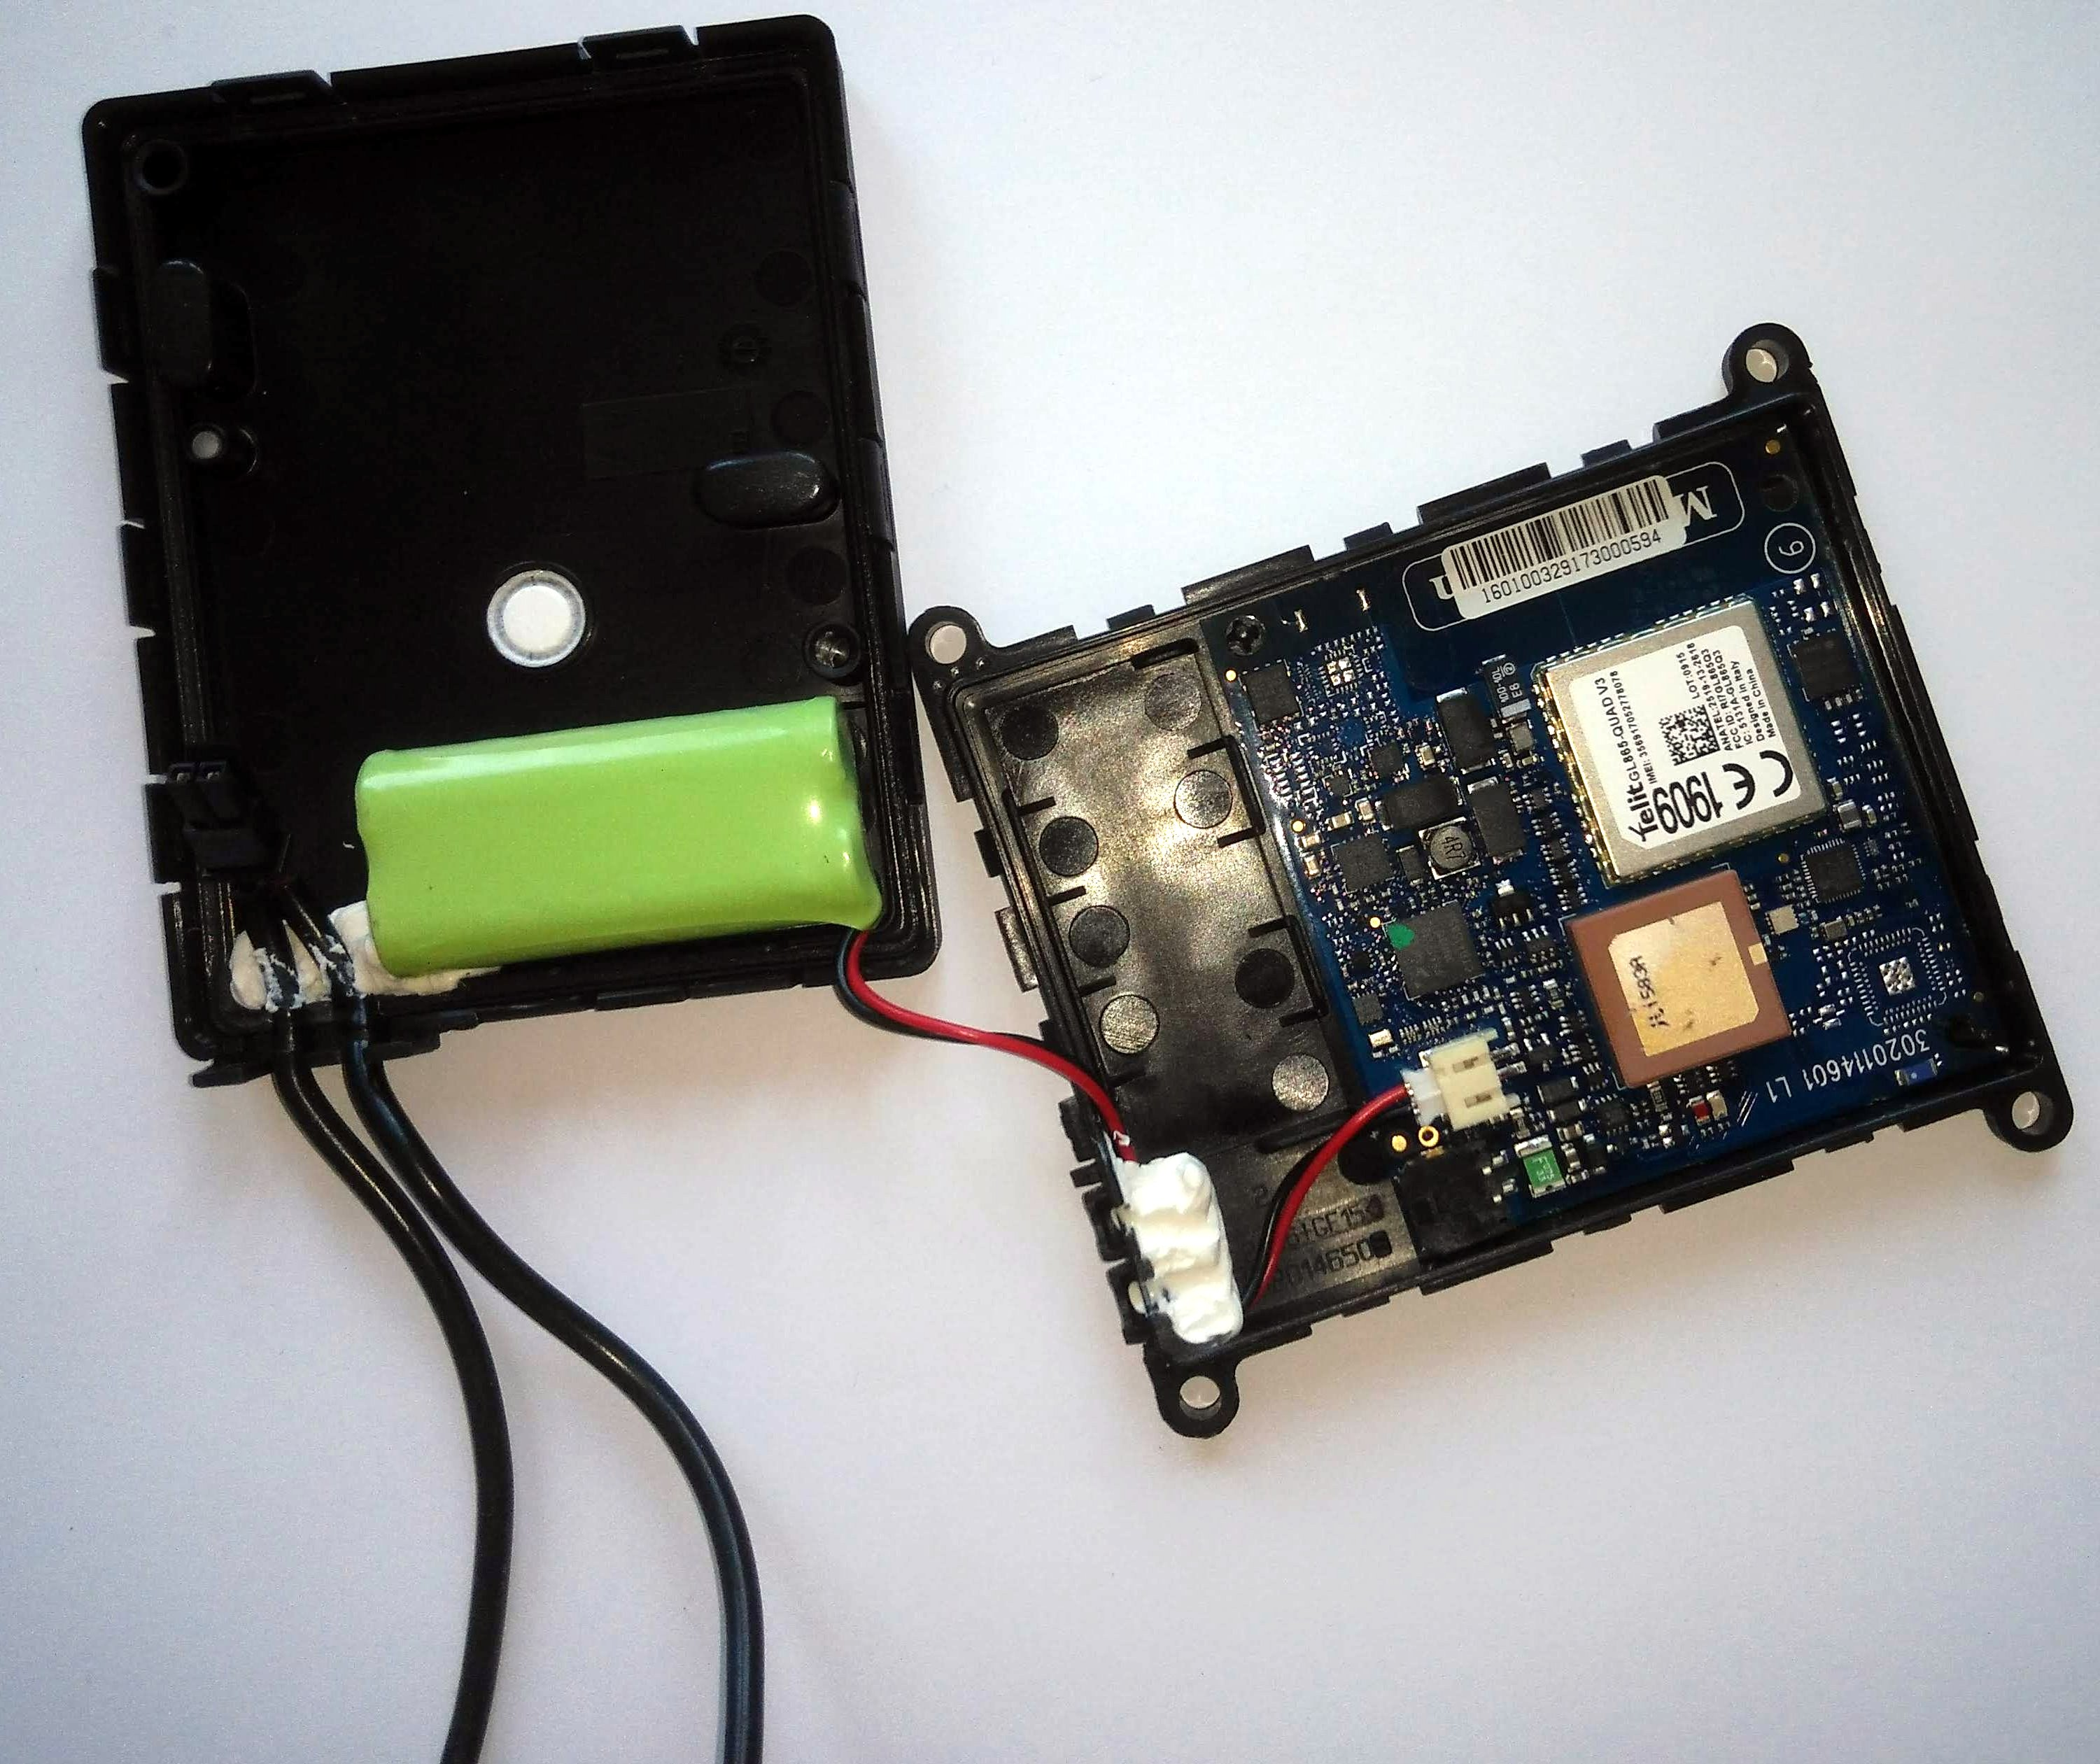
\includegraphics[width=\linewidth]{box.jpg}
\caption{One of the sensor box used to collect data}
\end{figure}

\justify
The experimental work will consist of verifying the possibility of creating a software capable of recreating a vehicle dynamic visually realistic.
The validation of results will be, in a first initial phase where effectiveness of the program will be low, exclusively visually empiric, because of the need of rapid development and testing times. In a second and later phase, when quality of output will become more difficult to evaluate empirically, results will be compared to pictures and video footages captured in the data acquisition phases. \\
\\
Aspiring software solution may face some challenges: sensor data gathering and transmission, correction of bad alignment, integration numerical error, precision reinforcement with multiple sensor fusion, representation of reconstructed trajectory. \\
\\
Input date format is specified in a Physycom(PHYsics of COMplex SYstem) group's Github online repository \footnote{\url{https://github.com/physycom/file_format_specifications/blob/master/formati_file.md}}. \\
I searched for an universal standard file format for inertial and GNSS data but I didn't find previous work. \\
\\	
Briefly formats supported by the software are all the following combinations:

\begin{center}
\begin{table}[H]
\begin{tabular}{l|l|l|}
\cline{2-3}
 & \textbf{inertial} & \textbf{inertial+GNSS} \\ \hline
\multicolumn{1}{|l|}{\textbf{interpolated}} & inertial & fullinertial \\ \hline
\multicolumn{1}{|l|}{\textbf{non interpolated}} & unmodified-inertial & unmodified-fullinertial \\ \hline
\end{tabular}
\end{table}

\end{center}

\justify
The \textit{full-inertial} format is the more complete one, containing both accelerometer, gyroscope and GNSS data. Indeed, the program will give a better output when provided with a \textit{full-inertial} input file, as it has more data to improve reconstruction. 
Records can be interpolated, in this case have always data from all sensors, instead of only from one of them, as they can have different frequencies. \\
In the case input data isn't interpolated, the software will take care of doing it. \\
\\
The following table shows \textit{full-inertial} data format in the order in which it is presented in the input files.

\begin{table}[H]
\begin{tabular}{|c|c|c|c|c|}
\hline
\begin{tabular}[c]{@{}c@{}}Dataset\\ Column\\ Index\end{tabular} & Name & Type & \begin{tabular}[c]{@{}c@{}}Unit\\ of\\ measure\end{tabular} & Notes \\ \hline
0 & Timestamp & Float & Seconds & From 1/1/2000 UTC+1 \\ \hline
1 & Latitude & Float & Degrees & From -90 to +90 \\ \hline
2 & Longitude & Float & Degrees & From -180 to +180 \\ \hline
3 & Altitude & Float & Meters & from sea level \\ \hline
4 & Heading & Float & Degrees & \begin{tabular}[c]{@{}c@{}}Measured from magnetic\\ north, from 0 to 360\end{tabular} \\ \hline
5 & Speed & Float & Km/h &  \\ \hline
6 & Acceleration X & Float & g-unit & Inertial \\ \hline
7 & Acceleration Y & Float & g-unit & Inertial \\ \hline
8 & Acceleration Z & Float & g-unit & Inertial \\ \hline
9 & Angular speed X & Float & Degrees/Seconds & \begin{tabular}[c]{@{}c@{}}right-handed \\ reference system\end{tabular} \\ \hline
10 & Angular speed Y & Float & Degrees/Seconds & \begin{tabular}[c]{@{}c@{}}right-handed \\ reference system\end{tabular} \\ \hline
11 & Angular speed Z & Float & Degrees/Seconds & \begin{tabular}[c]{@{}c@{}}right-handed \\ reference system\end{tabular} \\ \hline
12 & Acceleration module & Float & g-unit &  \\ \hline
13 & Relative time & Float & Seconds & From first record \\ \hline
\end{tabular}
\end{table}

\justify
Lastly, I decided to visualize the reconstructed trajectory animated on the 3D modeling software Blender. The decision is motivated by the fact that Blender is a popular open source software and has an API to interact with. Additionally, it's already used inside the research group and one of its member is a 3D-artist specialized on it.
%TODO talk abot blender popularity with google trends as source?
